%%%%%%%%%%%%%%%%%%%%%%%%%%%%%%%%%%%%%%%%%%%%%%%%%%%%%%%%%%%%%%%%%%%%%%%%%%%%%%%%
% Chapter 2: Conceptos
%%%%%%%%%%%%%%%%%%%%%%%%%%%%%%%%%%%%%%%%%%%%%%%%%%%%%%%%%%%%%%%%%%%%%%%%%%%%%%%%

%++++++++++++++++++++++++++++++++++++++++++++++++++++++++++++++++++++++++++++++
% \section{Visión estéreo}
% \label{2:sec:2}
% http://vision.deis.unibo.it/~smatt/Seminars/StereoVision.pdf
% http://www.cesfelipesegundo.com/revista/articulos2011/Guerrero,%20J.M.pdf

La visión estereoscópica o visión estéreo, es la técnica capaz de extraer
información tridimensional (profundidad) a partir de la posición relativa de un
objeto en imágenes bidimensionales al ser observado desde distintos ángulo por
dos o más cámaras separadas a una cierta distancia.

%+++++++++++++++++++++++++++++++++++++++++++++++++++++++++++++++++++++++++++++++
% \subsection{Calibración}

%+++++++++++++++++++++++++++++++++++++++++++++++++++++++++++++++++++++++++++++++
\subsection{Adquisición}

Usando dos cámaras, el procedimiento a seguir para la adquisición del entorno
es capturar dos imágenes de una misma escena, desde dos cámaras separadas
ligeramente. De esta forma, las imágenes obtenidas, también tendrán un pequeño 
desplazamiento entre sí.

De manera más formal, se obtiene que para cada imagen capturada por las
cámaras, un objeto está en puntos diferentes del plano. Esta triangulación
entre el punto P y Q y el origen de referencia, provocan una sensación de
profundidad. Mediante el sistema tradicional de una sola cámara, este punto
estaría en las mismas coordenadas.

\begin{figure}[!th]
  \begin{center}
    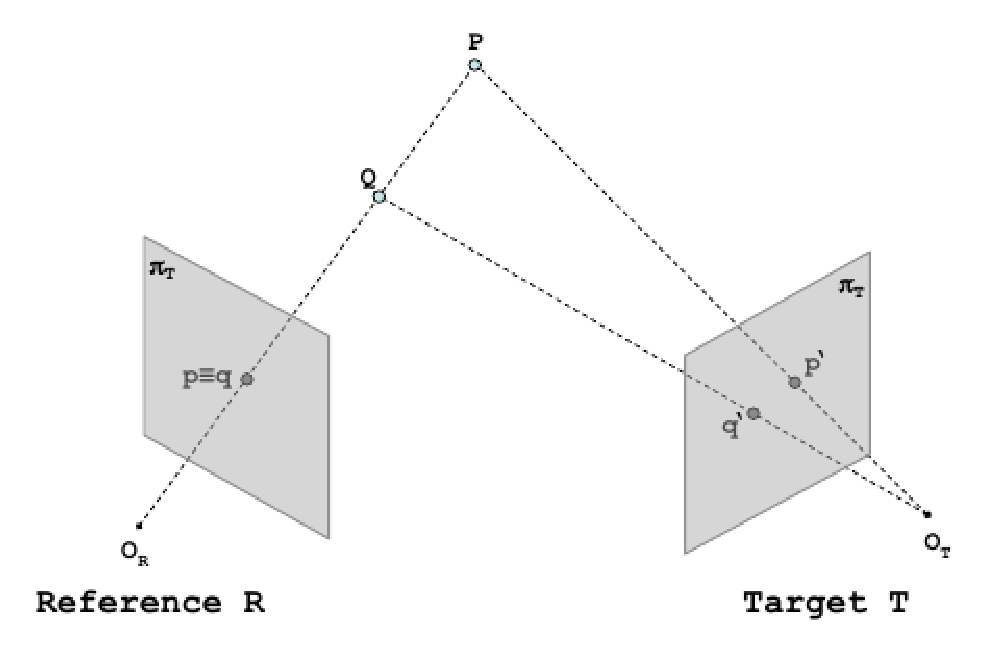
\includegraphics[width=0.5\textwidth]{images/cap2/VisionEstereo.eps}
    \caption{Diferencias entre una y dos cámaras}
    \label{fig:VisionEstereo}
  \end{center}
\end{figure}

Con estos datos, se pueden poner en correspondencia cada punto de ambas
imágenes, para obtener una imagen de disparidad (más información en la sección 
2.2.4).

%+++++++++++++++++++++++++++++++++++++++++++++++++++++++++++++++++++++++++++++++
\subsection{Geometría de las cámaras}
% https://en.wikipedia.org/wiki/Parallax
% http://www.cesfelipesegundo.com/revista/articulos2011/Guerrero,%20J.M.pdf
En función de la posición relativa de las cámaras entre sí, se pueden apreciar
dos métodos principales:

\begin{itemize}
  \item \textbf{Visión paralela:} las cámaras están paralelas entre sí y están
  separadas por una línea horizontal (línea base). El objetivo que visualiza
  cada cámara es perpendicular respecto a la línea base, mientras que las
  líneas de correspondencia que unen los puntos de una imagen respecto a la
  otra son horizontales.

  \begin{minipage}{\linewidth}
      \centering
      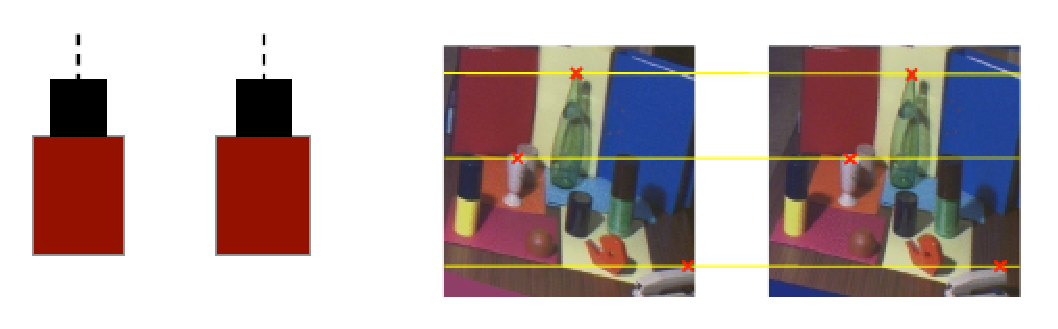
\includegraphics[width=0.6\textwidth]{images/cap2/VisionParalela.eps}
      \captionof{figure}{Visión paralela}
      \label{fig:VisionParalela}
  \end{minipage}

  \item \textbf{Visión cruzada:} las cámaras no están paralelas entre sí,
  tienen una inclinación de tal forma que el objetivo de cada cámara apunta
  hacia el lado contrario de una imagen. Por lo que los ejes ópticos se cruzan
  entre sí. Las líneas de correspondencia, también tienen sufren una
  inclinación.

  \begin{minipage}{\linewidth}
      \centering
      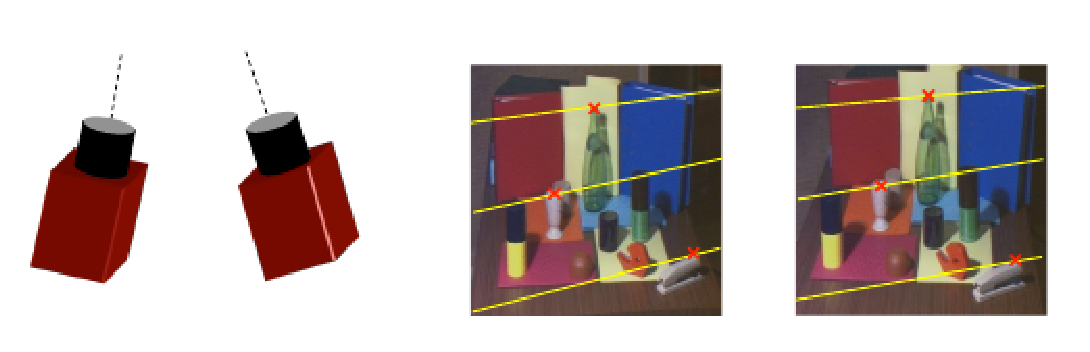
\includegraphics[width=0.6\textwidth]{images/cap2/VisionCruzada.eps}
      \captionof{figure}{Visión cruzada}
      \label{fig:VisionCruzada}
  \end{minipage}
\end{itemize}

% http://vfxio.com/PDFs/Parallel_vs_Converged.pdf
La visión cruzada tiene la desventaja de distorsionar las imágenes capturadas.
En la figura 2.4 se puede observar este efecto al fotografiar un muro de
ladrillos. Sin embargo, dependiendo del tipo de escena que se capture, esta
distorsión puede suponer un problema o no.

\begin{figure}[!th]
  \begin{center}
    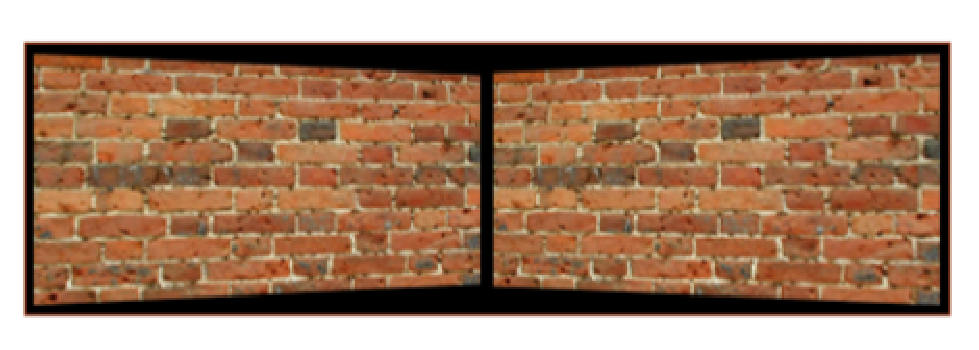
\includegraphics[width=0.5\textwidth]{images/cap2/VisionCruzadaMuro.eps}
    \caption{Muro distorsionado por visión cruzada}
    \label{fig:VisionCruzadaMuro}
  \end{center}
\end{figure}

La visión paralela por su parte, no distorsiona las imágenes capturadas, pero
también cuenta con otra serie de problemas. A pesar de ello, la visión paralela
suele ser la más utilizada para la visión estéreo.

%+++++++++++++++++++++++++++++++++++++++++++++++++++++++++++++++++++++++++++++++
% \subsection{Rectificación}
% https://en.wikipedia.org/wiki/Image_rectification

%+++++++++++++++++++++++++++++++++++++++++++++++++++++++++++++++++++++++++++++++
\subsection{Disparidad}
% http://es.slideshare.net/RicardoSnchezCastill/vision-artificial-49264591
% http://stackoverflow.com/questions/17607312/difference-between-disparity-map-and-disparity-image-in-stereo-matching
% http://iie.fing.edu.uy/publicaciones/2005/Lec05a/Lec05a.pdf
La disparidad de dos imágenes establece la correspondencia entre los píxeles o
características que existen entre ambas en el eje x para obtener la profundidad
de la escena. Con esto se consigue estimar la profundidad de cada uno de los
puntos en la escena.

El objetivo final es poder construir una \textbf{imagen o mapa de disparidad},
una imagen que representa la disparidad entre las dos cámaras. Habitualmente
el mapa de disparidad se representa como una imagen monocroma donde los objetos
con mayor disparidad (más cercanos) son representados con un tono más claro y
los objetos con menor disparidad (más lejanos) son representados con un tono más
oscuro. Aunque no es extraño encontrar una imagen térmica en vez de monocroma.

Con el único requisito de que las imágenes estén rectificadas, el algoritmo para
calcular la disparidad consiste de forma general en obtener la profundidad para
todos los píxeles de las imágenes estéreo. De esta forma, para todos los puntos
de cada imagen se busca la pareja de puntos correspondientes que representan la
proyección del mismo punto del espacio.

El mapa de disparidad es uno de los elementos básicos para la reconstrucción
tridimensional de los objetos de una escenas a partir de varias capturas.

\begin{figure}[!th]
  \begin{center}
    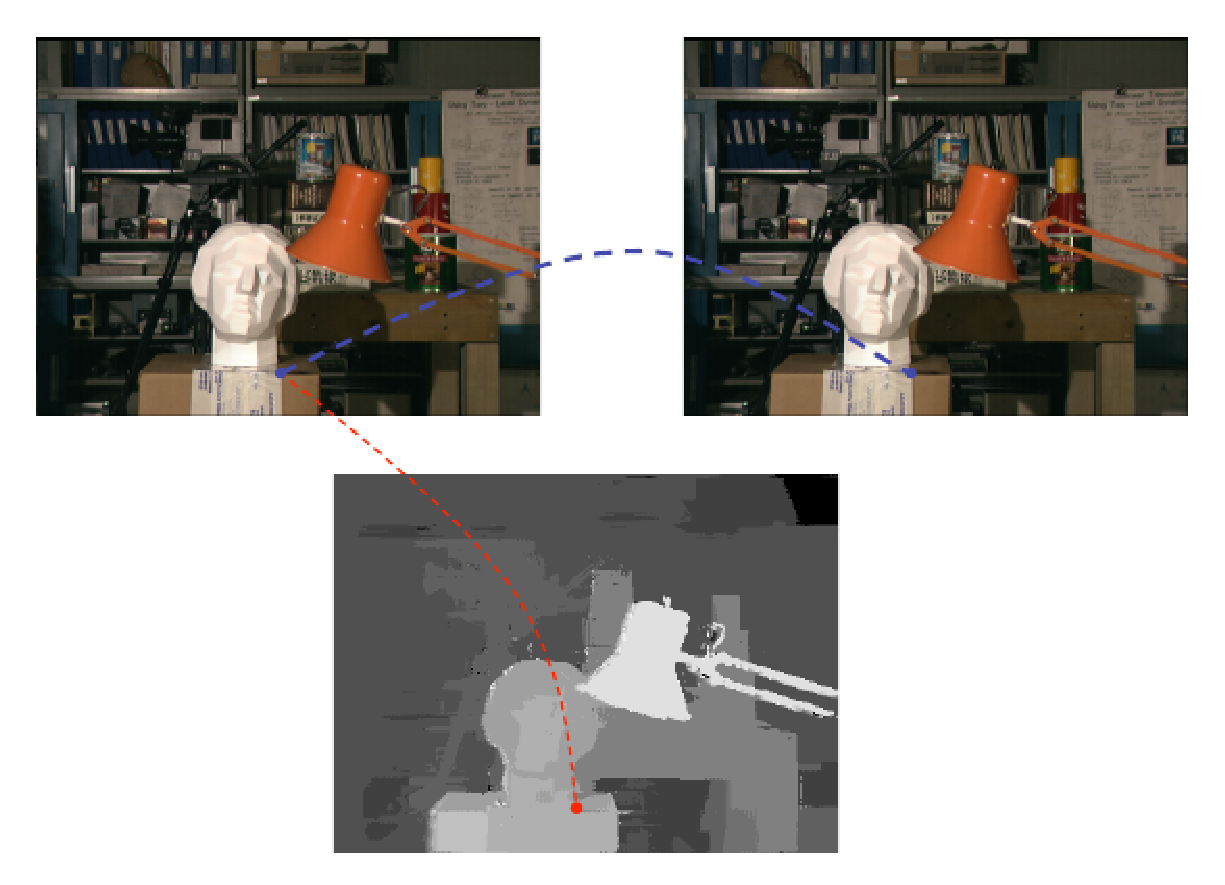
\includegraphics[width=0.6\textwidth]{images/cap2/MapaDisparidad.eps}
    \caption{Mapa de disparidad a partir de imágenes en estéreo}
    \label{fig:MapaDisparidad}
  \end{center}
\end{figure}


% Disparidad....

% http://www.cesfelipesegundo.com/revista/articulos2011/Guerrero,%20J.M.pdf
% http://dmi.uib.es/~abasolo/cursorealidad/paco/Estereoscopia.html


%+++++++++++++++++++++++++++++++++++++++++++++++++++++++++++++++++++++++++++++++
% \subsection{Reconstrucción 3D}

%++++++++++++++++++++++++++++++++++++++++++++++++++++++++++++++++++++++++++++++
